% Standalone RAKL transfer-decision flowchart (Paper II).
% Non-compensatory applicability gate: LICENSED / REJECTED / CANNOT_CHECK.
% Build:  pdflatex transfer_decision.tex  -> transfer_decision.pdf
\documentclass[border=6pt]{standalone}
\usepackage{tikz}
\usepackage{helvet}\renewcommand{\familydefault}{\sfdefault}
\usetikzlibrary{positioning,arrows.meta,shapes.geometric,fit,backgrounds,calc}
\definecolor{oiblue}{RGB}{0,114,178}
\definecolor{oiverm}{RGB}{213,94,0}
\begin{document}
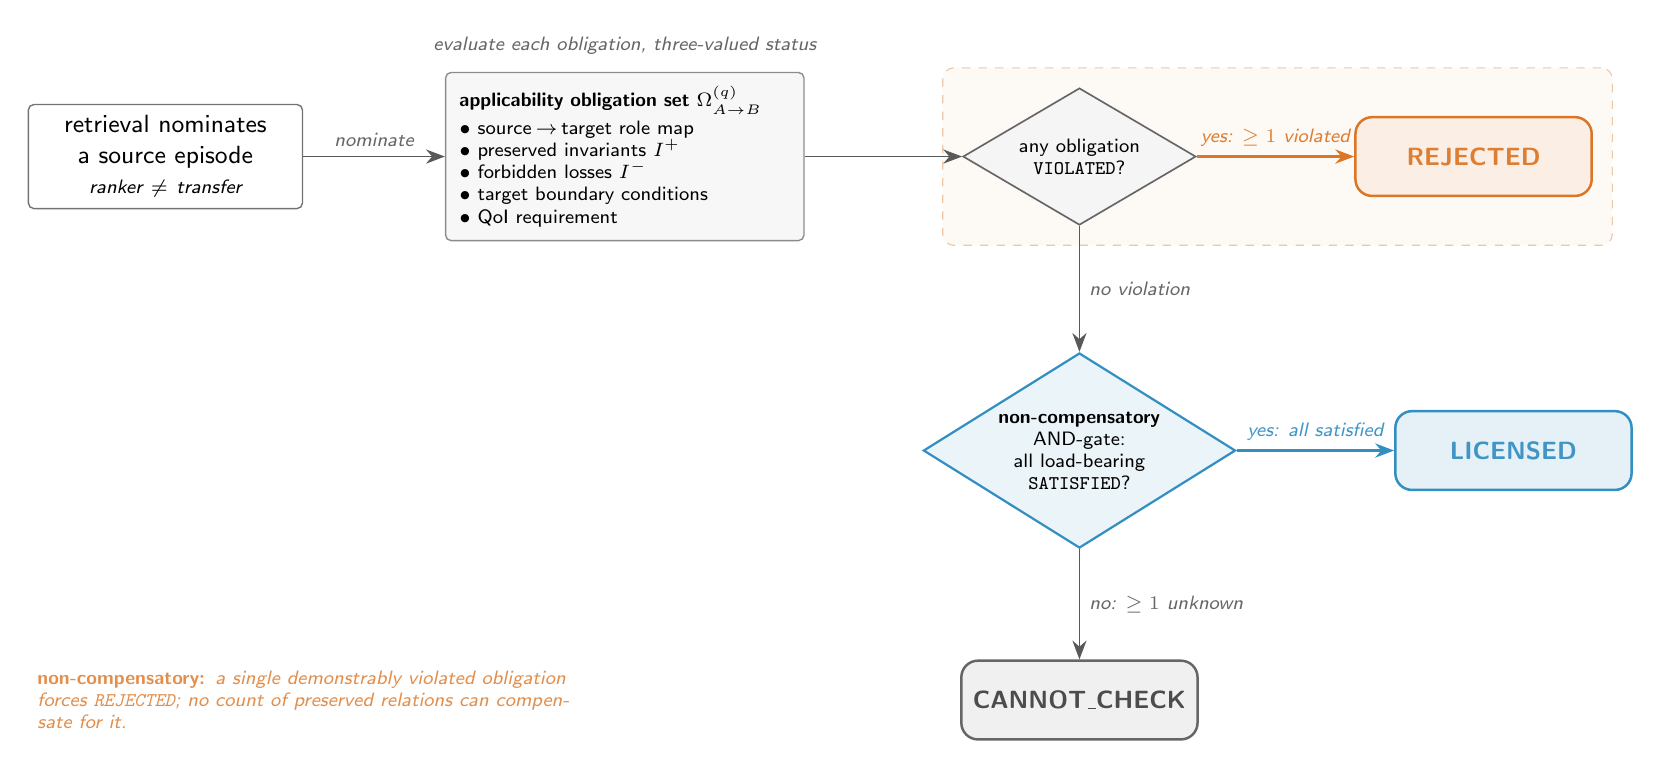
\begin{tikzpicture}[
  font=\small,
  >={Stealth[length=2.4mm]},
  proc/.style={rounded corners=2pt, draw=black!55, line width=0.5pt, align=center,
               inner sep=4pt, minimum height=9mm, minimum width=26mm, fill=white},
  obox/.style={rounded corners=2pt, draw=black!45, line width=0.5pt, align=left,
               inner sep=5pt, fill=black!3, text width=42mm, font=\scriptsize},
  gate/.style={diamond, aspect=1.6, draw=oiblue!80, line width=0.8pt, align=center,
               inner sep=1pt, fill=oiblue!8, font=\scriptsize},
  dec/.style={diamond, aspect=1.7, draw=black!60, line width=0.6pt, align=center,
              inner sep=1pt, fill=black!4, font=\scriptsize},
  license/.style={rounded corners=6pt, draw=oiblue!80, line width=0.9pt, align=center,
               inner sep=4pt, minimum height=10mm, minimum width=30mm, fill=oiblue!10,
               font=\small\bfseries, text=oiblue!75},
  reject/.style={rounded corners=6pt, draw=oiverm!85, line width=0.9pt, align=center,
               inner sep=4pt, minimum height=10mm, minimum width=30mm, fill=oiverm!10,
               font=\small\bfseries, text=oiverm!80},
  abstain/.style={rounded corners=6pt, draw=black!60, line width=0.9pt, align=center,
               inner sep=4pt, minimum height=10mm, minimum width=30mm, fill=black!6,
               font=\small\bfseries, text=black!70},
  flow/.style={->, line width=0.6pt, draw=black!65},
  lbl/.style={font=\scriptsize\itshape, text=black!60},
  node distance=9mm and 16mm,
]
% ---- retrieval nominates a source ----
\node[proc, text width=32mm] (ret) {retrieval nominates\\a source episode\\{\scriptsize\itshape ranker $\neq$ transfer}};

% ---- applicability obligation checklist ----
\node[obox, right=18mm of ret] (checklist)
  {\textbf{applicability obligation set} $\Omega_{A\to B}^{(q)}$\\[2pt]
   $\bullet$ source$\,\to\,$target role map\\
   $\bullet$ preserved invariants $I^{+}$\\
   $\bullet$ forbidden losses $I^{-}$\\
   $\bullet$ target boundary conditions\\
   $\bullet$ QoI requirement};
\node[lbl, above=1mm of checklist] {evaluate each obligation, three-valued status};

% ---- per-obligation status classifier ----
\node[dec, right=20mm of checklist, text width=20mm] (status)
  {any obligation\\ \texttt{VIOLATED}?};

% ---- non-compensatory AND-gate (only when nothing violated) ----
\node[gate, below=16mm of status, text width=22mm] (andgate)
  {\textbf{non-compensatory}\\AND-gate:\\all load-bearing\\ \texttt{SATISFIED}?};

% ---- outcomes ----
\node[reject, right=20mm of status] (rej) {REJECTED};
\node[license, right=20mm of andgate] (lic) {LICENSED};
\node[abstain, below=14mm of andgate] (cc) {CANNOT\_CHECK};

% ---- edges ----
\draw[flow] (ret) -- node[lbl,above]{nominate} (checklist);
\draw[flow] (checklist) -- (status);

% VIOLATED -> REJECTED (any single violation forces rejection)
\draw[flow, draw=oiverm!85, line width=0.9pt]
   (status) -- node[lbl,above,text=oiverm!80]{yes: $\ge 1$ violated} (rej);
% not violated -> AND-gate
\draw[flow] (status) -- node[lbl,right]{no violation} (andgate);

% AND-gate: all satisfied -> LICENSED
\draw[flow, draw=oiblue!80, line width=0.9pt]
   (andgate) -- node[lbl,above,text=oiblue!75]{yes: all satisfied} (lic);
% AND-gate: some UNKNOWN -> CANNOT_CHECK
\draw[flow] (andgate) -- node[lbl,right]{no: $\ge 1$ unknown} (cc);

% ---- non-compensatory annotation band ----
\begin{scope}[on background layer]
  \node[draw=oiverm!35, dashed, rounded corners=4pt, fill=oiverm!4,
        fit=(status)(rej), inner sep=7pt] (ncbox) {};
\end{scope}
% caption placed in the open lower-left region so it clears every edge label
\node[font=\scriptsize\itshape, text=oiverm!70, align=left, text width=68mm,
      anchor=west] at (ret.west |- cc)
  {\textbf{non-compensatory:} a single demonstrably violated obligation forces
   \texttt{REJECTED}; no count of preserved relations can compensate for it.};

\end{tikzpicture}
\end{document}
